% --------------------------------------------------------------------

\chapter[Variable Objects]{Variable Objects}
\def\chpname{variables}\label{chp:\chpname}

Chapter editors:
\credit{AshishMahabal},
\credit{lmwalkowicz}.

Contributing authors:
\credit{lundmb},
\credit{StephenRidgway},
\credit{keatonb},
\credit{phartigan},
\credit{CJohnsKrull},
\credit{pmmcgehee},
\credit{ShashiKanbur}

% \section*{Summary}
% \addcontentsline{toc}{section}{~~~~~~~~~Summary}
%
% Executive summary goes here, highlighting the primary conclusions from
% the chapter's science cases. This should be abstract length, no more:
% say, 200 words.

% --------------------------------------------------------------------


\section{Introduction}

Variable objects are defined as those that exhibit brightness changes,
either periodic or non-periodic, which are detected in quiescence and
non-destructive to the object itself. Variable objects span a wide range
in timescale-of-interest (sometimes even within a single class of
objects), and so different science cases benefit from different sampling
strategies. These strategies may be significantly disparate from one
another, sometimes even mutually exclusive; competing objectives
described in this chapter and the next are therefore at the heart of
LSST observing strategy and cadence design.

Below we develop a number of key science cases for LSST studies of
variable objects, associating them with related metrics that can be used
within the Metrics Analysis Framework (MAF) to understand the impact of
a given survey strategy realization on the scientific results for that
case. The science cases outlined are by no means exhaustive, but rather
are motivated by providing key quantitative examples of LSST's
performance given any particular deployment of survey strategy. The
authors encourage community contribution of similar cases, where the
scientific outcome can be quantified using specific metrics.



%When evaluating a particular observation or series of observations in
%light of how they perform for a specific science case, it may be
%helpful to think of metrics as lying along a continuum between
%discovery and characterization. Discovery requires a minimum amount of
%information to recognize an event or object as a candidate of
%interest, which necessarily involves some level of bare-bones
%characterization (upon which said recognition is based); rich
%characterization, on the other hand, implies that an event may not
%only be recognized as a candidate of interest, but basic properties of
%the event or object may be determined from the observation (e.g.
%including but not limited to classification of the event). The
%interpretation of a given metric along this continuum has implications
%for the subsequent action and analysis required, particularly as
%regards possible follow-up observations with other facilities.

%Target types are here grouped in subsections by variability
%characteristics, but as will be seen, this does not mean that all
%targets in a group require a common cadence, since the times scales
%may vary dramatically.  Acquiring suitable data for a wide range of
%time scales presents a fundamental problem for LSST, since the
%available $~$800 visits to a field over the survey cannot be deployed
%so as to usefully sample all time scales at all times.  This fact
%leads to the concept of a non-uniform survey, in which parts of the
%sky are visited more frequently part of the time.  The merits of such
%options must be traded against the benefits of a more uniform survey
%strategy.

\begin{center}
\begin{tabular}{| l | p{8cm} |l | l |}
\hline Periodic Variable Type & Examples of target science & Amplitude & Timescale\\
\hline
RR Lyrae & Galactic structure, distance ladder, RR Lyrae properties&  large &  day \\
Cepheids & Distance ladder, cepheid properties&  large &  day \\
Long Period Variables & Distance ladder, LPV properties & large  &  weeks \\
Short period pulsators & Instability strip, white dwarf interior properties, evolution&  small & min  \\
Periodic binaries & Eclipses, physical properties of stars, distances, ages, evolution, apsidal precession, mass transfer induced period changes, Applegate effect &  small &  hr-day \\
Rotational Modulation & Gyrochronology, stellar activity & small  &  days \\
Young stellar populations & Star and planet formation, accretion physics & small  &  min-days \\
 \hline \end{tabular}
 \end{center}


% --------------------------------------------------------------------

% ====================================================================
%+
% SECTION:
%    cepheids.tex
%
% CHAPTER:
%    variables.tex
%
% ELEVATOR PITCH:
%
%-
% ====================================================================

\section{The Cepheid Mass-Luminosity Relation}
\def\secname{cepheids}\label{sec:\secname}

Classical Cepheids begin to pulsate once they evolve up the giant branch and
execute blueward loops on the HR diagram that take them into the Instability
Strip. Cepheid masses and luminosities in the instability strip are connected
through the Mass-Luminosity (ML) relation.  This ML relation is strongly
dependent on stellar evolution physics. Canonical/Non-canonical ML relations
arise from varying treatments of convective core overshoot and mass loss
\citep{1992A&A...258..397B,2000ApJ...529..293B,2013ApJ...768L...6M}.

Stellar pulsation models adopt a given ML relation and then compute a
theoretical light curve for a range of different temperatures and
metallicities. This theoretical light curve can then be transformed into LSST
wavebands using stellar atmospheres (\citep{Bono2000} and references therein) and
quantitatively compared to observed LSST light curves through Fourier
decomposition of the form
$$V = A_0 + \sum_{k=1}^{k=N}A_k cos(k\omega t + {\phi}_k),$$
where $\omega = 2\pi/P,$ with $P$ the period, $N$ is the order of the fit. The
coefficients $R_{k1}=A_k/A_1$ and ${\phi}_{k1}={\phi}_k - k{\phi}_1$ can be
computed for both theoretical and LSST observed light curves. These
coefficients are sensitive to the adopted $ML$ relation and other global
parameters such as metallicity and effective temperature.  By utilizing such a
decomposition, the multiwavelength light curves that the LSST will produce for
both Cepheids and RR Lyraes can rigorously constrain Cepheid and RR Lyrae
global stellar parameters such as the ML relation. Of course, knowledge of the
ML relation through this approach can then lead to another ``theoretical''
distance scale using both Cepheids and RR Lyraes.  However, in the case of
Cepheids, given good enough cadence in LSST bands and thus an accurate Fourier
decomposition with precisely known Fourier parameters, it will be possible to
discriminate between canonical and non-canonical ML relations and thus provide
constraints for stellar evolution physics. {\it A good Figure of Merit for
this science case would be one based on the precision with which
we can infer the parameters of these relations.}

\citet{2014MNRAS.445.2655B} describes in detail the way the quantitative structure of
Cepheid and RR Lyrae light curves vary with period and optical band. Given
appropriate cadence, LSST light curves will provide accurate Fourier
decompositions at multiple wavelengths that can significantly augment these
results and provide an important database with which to connect quantitative
aspects of Cepheid and RR Lyrae light curve structure to pulsation envelope
physics. Two examples are the following.
\begin{itemize}
\item{1)} RRab stars found in stripe 82 of the
SDSS exhibit a flat Period-Color (PC) relation at minimum light at certain SDSS colors but not at others. LSST observations of RRab stars will be able
to augment this result and investigate if there are any links to the structural properties of observed light curves.
\item{2)} Short period ($\log P \le 0.4$) FU Cepheids in the SMC exhibit a noticeable break in their $(V-I)$ PC relation at certain phases of pulsation
phases. At the same period, the Fourier parameter $R_{21}$ displays a strong turnover. LSST data will be important in seeing if this result extends
to LSST colors.
\end{itemize}

\citet[and references therein]{2014MNRAS.445.2655B,2015MNRAS.447.3342B} have
demonstrated how Cepheid and RR Lyrae
Period-Color(PC)/Period-Luminosity (PL)/
Period-Wesenheit(PW)/Period-Luminosity-Color(PLC) relations vary significantly
both as a function pulsation phase and period and observation band.  The LSST
database on Cepheids and RR Lyraes will provide an excellent database to further
investigate the variation of these relations with pulsation phase with a view
to understanding pulsation physics and constraining theoeretical models.
Currently, the literature only discusses these relations at mean light, that
is the average over pulsation phase. Yet this averaging process masks
some dependencies: there are pulsation phases with very high/low PL/PC
dispersion and there are some phases where the relation is highly nonlinear.
In the era of precision cosmology, it is important to understand the tools that
we use to construct a distance scale. The LSST database on Cepheids and RR
Lyraes will be an important database with which to investigate the multiphase
properties of PL/PC/PW/PLC relations.

What cadence is required for ``accurate multiwavelength Fourier
decomposition''? Cepheids and RR Lyraes are strictly periodic. Then for known variables, whose periods are already known, such
Fourier decompositions can be carried out on folded light curves. In such
situations given a cadence, one possible measure of the success of this Fourier
decomposition could be the maximum phase gap in the folded light curve. Another
measure could be the error on the Fourier parameters
\citep{1986A&A...170...59P}. One way forward is to carry out a detailed
Fourier analysis of any one simulated schedule.

\subsection{Description of Relevant Metrics}
\label{sec:\chpname:variablemetrics}

Despite the range in scientific motivation for the cases presented
in this chapter,
there are some common metrics that are widely applicable (or may
be combined in a variety of ways with other metrics to suit a variety of
applications).
\new{The present science case provides as good a venue as
any in which to introduce these common metrics.}

%\subsection{Metrics}
%\label{sec:\chpname:metrics}

\begin{center}
\begin{tabular}{| p{5cm} |p{10cm} |}
\hline Metric & Description\\
\hline
Eclipsing/transiting system discovery & Fraction of discoveries vs fractional duration of eclipse\\
Lightcurve shape recovery & ... \\
%Transiting exoplanets (depth dependent) & Fraction of discoveries vs fractional duration of eclipse\\
Phase gap & Histogram vs period of the median and maximum phase gaps achieved in all fields\\
Period determination (period dependent) & Fraction of targets vs survey duration, for which the period can be determined to 5-sigma confidence\\
Period variability (period dependent) & Fraction of targets vs survey duration, for which a period change of 1\% can be determined with 5-sigma confidence\\
  \hline \end{tabular}
 \end{center}

The ability to identify that an object is periodic, and to correctly
determine that object's period, are widely applicable measures of
discovery. In the case of regular variables (as outlined below), these
two measures together can uniquely identify a population. Other kinds of
periodic systems (transiting planets for example) also require a
measurement of periodicity, but have a much wider range of relevant
periods, and looser requirements on the strictness of that periodicity.

\citet{LundEtal2016} discuss three {\it diagnostic} metrics that have been
incorporated into the MAF. Two of these metrics deal explicitly with time
variable behavior: a) observational triplets, and b) detection of periodic
variability.

%%%%%%%%%%%%%%%%%%%%%%%%%%%%%%%%%
\begin{figure}[tbh!]
%\vskip -4.1in
%\hskip -0.5in
%\includegraphics[angle=0,width=1.19\hsize:,clip]{figs/enigma1189_earlySNe.pdf}
%\vskip -4.0in
\includegraphics{figs/variables/enigma_1189_PeriodogramPurity_OPSI_SkyMap.pdf}
\caption{The value for the Periodogram Purity Function for candidate
Baseline Cadence \opsimdbref{db:baseCadence}. The Periodogram Purity
Function provides a measure of the power lost due to aliasing.}
\label{fig:enigmaPeriodogramPurity}
\end{figure}
%%%%%%%%%%%%%%%%%%%%%%%%%%%%%%%%%


%%%%%%%%%%%%%%%%%%%%%%%%%%%%%%%%%
\begin{figure}[tbh!]
%\vskip -4.1in
%\hskip -0.5in
%\includegraphics[angle=0,width=1.19\hsize:,clip]{figs/enigma1189_earlySNe.pdf}
%\vskip -4.0in
\includegraphics{figs/variables/enigma_1189_Phase_Gap_MedianGap_OPSI_SkyMap.pdf}
\caption{The median phase gap for candidate Baseline Cadence \opsimdbref{db:baseCadence}.
The PhaseGapMetric looks at periods between 3 and 35 days by default.}
\label{fig:enigmaMedianGap}
\end{figure}
%%%%%%%%%%%%%%%%%%%%%%%%%%%%%%%%%

%%%%%%%%%%%%%%%%%%%%%%%%%%%%%%%%%
\begin{figure}[tbh!]
%\vskip -4.1in
%\hskip -0.5in
%\includegraphics[angle=0,width=1.19\hsize:,clip]{figs/enigma1189_earlySNe.pdf}
%\vskip -4.0in
\includegraphics{figs/variables/enigma_1189_Phase_Gap_LargestGap_OPSI_SkyMap.pdf}
\caption{The maximum phase gap for candidate Baseline Cadence \opsimdbref{db:baseCadence}.
The PhaseGapMetric looks at periods between 3 and 35 days by default.}
\label{fig:enigmaMaxGap}
\end{figure}
%%%%%%%%%%%%%%%%%%%%%%%%%%%%%%%%%

\subsubsection{Periodogram purity function (PeriodicMetric)}

This metric calculates the Fourier power spectral window function of each field
\citep{1987AJ.....93..968R} as a means of quantifying the completeness of phase
coverage for a given periodic variable. The periodogram purity is defined as 1
minus the Fourier power spectral window function. in the perfect case, all
power in the window function is concentrated in a delta function at zero, and
is zero at all other frequencies. As power ``leaks'' away from the correct
frequency as a consequence of discrete, non-ideal data sampling, the
periodogram becomes more structured. For the purposes of MAF metrics, which are
designed to quantify performance as a single number, the periodogram purity is
quantified as the minimum value of the periodogram purity function at non-zero
frequency shifts; the ideal case would be a periodogram purity metric value of
1.

\subsubsection{Phase Gap Metric (PhaseGapMetric)}

The Phase Gap Metric is designed to examine the largest phase gaps in
the observing schedule. For a given point in the sky, a series of
periods are randomly selected (by default, 5 periods), with a default
minimum of 3 days and maximum of 35 days. The largest phase gap for each
period is calculated, and the metric plots the median
(\autoref{fig:enigmaMedianGap}) and maximum (\autoref{fig:enigmaMaxGap})
of this subset of values that contains the maximum phase gap per period.
The Phase Gap Metric is part of varMetrics.

\subsubsection{Period Deviation Metric (PeriodDeviationMetric)}

The Period Deviation Metric calculates the error in recovering the
correct period of a sinusoid using a given observing schedule and a
Lomb-Scargle periodogram. For a given point in the sky, a series of
periods are randomly selected (by default, 5 periods), and the metric
returns the worst period deviation, and the period at which this
occurred. The Period Deviation Metric is part of varMetrics.

%\subsection{Proposed Metrics}

%The following is a raw list of metric ideas; these need specificity and further description.

%FWHM of the window function (to quantify sampling)

%Maximum hour angle difference

%Fraction of discoveries vs fractional duration of eclipse

%Fraction of targets vs survey duration, for which the period can be determined to 5-sigma confidence

%Fraction of targets vs survey duration, for which a period change of 1$\%$ can be determined with 5-sigma confidence

% ====================================================================
%
% \subsection{OpSim Analysis}
%
% ====================================================================
%
 \subsection{Conclusions}

 Here we answer the ten questions posed in
 \autoref{sec:intro:evaluation:caseConclusions}:

 \begin{description}

 \item[Q1:] {\it Does the science case place any constraints on the
 tradeoff between the sky coverage and coadded depth? For example, should
 the sky coverage be maximized (to $\sim$30,000 deg$^2$, as e.g., in
 Pan-STARRS) or the number of detected galaxies (the current baseline but
 with 18,000 deg$^2$)?}

 \item[A1:] Cepheid light curves will be well sampled with far less than the ~800 visits acquired in the baseline survey, hence increased sky coverage would measure cepheids in a larger number of galaxies, which would be valuable.

 \item[Q2:] {\it Does the science case place any constraints on the
 tradeoff between uniformity of sampling and frequency of  sampling? For
 example, a rolling cadence can provide enhanced sample rates over a part
 of the survey or the entire survey for a designated time at the cost of
 reduced sample rate the rest of the time (while maintaining the nominal
 total visit counts).}

 \item[A2:] An enhanced cadence could provide earlier discovery and period confirmation for a subset of targets, but this is
not a high priority.

 \item[Q3:] {\it Does the science case place any constraints on the
 tradeoff between the single-visit depth and the number of visits
 (especially in the $u$-band where longer exposures would minimize the
 impact of the readout noise)?}

 \item[A3:] No strong constraint.

 \item[Q4:] {\it Does the science case place any constraints on the
 Galactic plane coverage (spatial coverage, temporal sampling, visits per
 band)?}

 \item[A4:] LSST observations of galactic cepheids are not high priority, since they are bright for LSST.

 \item[Q5:] {\it Does the science case place any constraints on the
 fraction of observing time allocated to each band?}

 \item[A5:] No strong constraint as long as good representation of all.

 \item[Q6:] {\it Does the science case place any constraints on the
 cadence for deep drilling fields?}

 \item[A6:]  This would only apply in deep drilling fields that were chosen to study relatively near-by galaxies, for which cepheid 
optimization would no doubt be considered explicitly.

 \item[Q7:] {\it Assuming two visits per night, would the science case
 benefit if they are obtained in the same band or not?}

 \item[A7:] Different bands would provide more rapid characterization of targets, but this is not a strong benefit.

 \item[Q8:] {\it Will the case science benefit from a special cadence
 prescription during commissioning or early in the survey, such as:
 acquiring a full 10-year count of visits for a small area (either in all
 the bands or in a  selected set); a greatly enhanced cadence for a small
 area?}

 \item[A8:]  Enhanced cadences could provide earlier science, but 
cepheids are not a strong driver for this.

 \item[Q9:] {\it Does the science case place any constraints on the
 sampling of observing conditions (e.g., seeing, dark sky, airmass),
 possibly as a function of band, etc.?}

 \item[A9:] No constraints that are particular to cepheids, but good seeing will aid the study of stars in the crowded fields of 
external galaxies.

 \item[Q10:] {\it Does the case have science drivers that would require
 real-time exposure time optimization to obtain nearly constant
 single-visit limiting depth?}

 \item[A10:] No.

 \end{description}


% --------------------------------------------------------------------

% PJM: moved to Future Work while MAF analysis is pending:
% 
% ====================================================================
%+
% SECTION:
%    periodicpulsators.tex
%
% CHAPTER:
%    variables.tex
%
% ELEVATOR PITCH:
%
%-
% ====================================================================

% \section{Discovery of Periodic Pulsating Variables}
\subsection{Discovery of Periodic Pulsating Variables}
\def\secname{periodicvariables}\label{sec:\secname}

\credit{lmwalkowicz},
\credit{StephenRidgway}

Regular variables, such as Cepheids and RR Lyraes, are valuable tracers
of Galactic structure and cosmic distance. In this case of these and
other strictly (or nearly-strictly) periodic variables, data from
different cycles of observation can be phase-folded to create a more
fully sampled lightcurve as LSST visits will occur effectively at random
phases. In a 10-year survey, most periodic stars of almost any period
will benefit from excellent phase coverage in all filters (only a very
small period range close to the sidereal day will be poorly observed).
Therefore, most implementations of the LSST observing strategy will
provide good sampling of periodic variables.

However, different implementations of the survey may result in different
resulting sample sizes of these periodic variables, and may also affect
the environments in which these stars are discovered. In this section,
we create a framework for understanding how current implementations of
the observing strategy influence (or even bias) the resultant sample
size and environments where these important tracers may be identified.

\subsubsection{Tracing Galactic Structure with RR Lyrae}

RR Lyrae variables are crucial tracers of structure in the Galaxy and beyond
into the Local Group. The incredible sample of RR Lyrae anticipated from LSST
observations will enable discovery of Galactic tidal stream and neighboring
dwarf galaxies throughout much of the Local Group
\citep{IvezicEtal2008}.  LSST also creates the possibility
of detecting and studying RRL variables in the Magellenic Clouds; see Chapter
[CHAPTER] for discussion.

\citet{2012AJ....144....9O} carried out an extensive simulation of period
and lightcurve shape recovery of RR Lyrae variables using an early OpSim run
opsim1$\_$29. Correctly identifying the period aids in building the sample of
interest, whereas fitting the lightcurve shape makes it possible to measure the
metallicity of the star. In their simulation, they employed both a Fourier
analysis and template matching to recover the lightcurve shape, finding that
template matching yielded a more accurate lightcurve shape measurement in the
presence of sparse data. The results of this simulation showed that the vast
majority of RR Lyrae will be discovered by the baseline observing strategy (as
deployed in opsim1$\_$29) within 5 years of survey operations. Half of both
RRLab and RRLc stars will be found out to $\sim$600 kpc and $\sim$250 kpc
(respectively) by the end of the 10-year main survey, and template matching
techniques for lightcurve shape recovery will provide metallicities to
$\sim$0.15dex.

% --------------------------------------------------------------------

\subsubsection{The Cepheid Cosmic Distance Ladder}

Classical cepheids remain an essential step in the cosmic distance
ladder. Their calibration is based largely on LMC cepheids and known
(assumed) distance of the LMC.  The associated errors, while uncertain,
are believed to be of $\>\sim$7\%. (Madore, Barry F.; Freedman, Wendy L.
(2009). "Concerning the Slope of the Cepheid Period?Luminosity
Relation". The Astrophysical Journal 696 (2): 1498. arXiv:0902.3747.
Bibcode:2009ApJ...696.1498M. doi:10.1088/0004-637X/696/2/1498.) New
developments in galactic studies are poised to support substantially
improved descriptive information concerning nearby galactic cepheids,
with possible substantial reductions in this error, by accurately
securing the PL slope and zero point.

Cepheid calibration errors are associated in part with uncertainties in
extinction, both interstellar and in some cases circumstellar, and in
metalicity.  At present, the direct, local calibration of cepheids is limited
by the availability of a few direct distance measurements, obtained with HST,
with errors $\sim$10\%.  The GAIA mission is expected to return $\sim$9000
Galactic cepheids, of all periods, colors and metallicities, with distance
errors less than 10\% (many of them much less) - Windmark, F.; Lindegren, L.;
Hobbs, D., 2011A\&A...530A..76W. It is expected to deliver at least 1000
cepheids in the LMC with expected mean distance error $\sim$7-8\% (Clementini
(2010) - 011EAS....45..267C).  GAIA, as well as other methods, will also
support determination of the 3-d map of galactic interstellar extinction -
including possible variations in the extinction law. These rich data sets will
be supported with direct measurements of cepheid diameters (A. Merand et al,
A\&A in press) and advances in stellar hydrodynamics
\citep{2013MNRAS.435.3191M} which will provide theoretical and empirical basis
for calibrations to reconcile known physics with observational correction
factors.

Galactic cepheids will generally be too bright for LSST, but cepheids in
the local group are sufficiently bright that LSST photometry will be
limited by calibration errors rather than by brightness.  This dataset
will provide superb support for integration of GAIA-based galactic
cepheid studies with extra-galactic cepheid studies.

GAIA will provide similar precision data with the potential to identify
or support distance determinations from many other galactic star types.
LSST photometric catalogs will represent a uniquely extensive and
complete database for such investigations.

% --------------------------------------------------------------------

% \subsection{Metric Analysis}
\subsubsection{Metric Analysis}
\label{sec:\secname:analysis}

Several metrics currently exist in the MAF for evaluating how LSST
survey strategy affect the recovery of periodic sources.
For example,
the PeriodicMetric makes use of the periodogram purity function, which effectively
quantifies aliasing introduced into periodogram analysis from the
sampling of the lightcurve.
%
% and period deviation metric (PeriodDeviationMetric) all return relevant
% information
%
Similarly, the
phase gap metric (PhaseGapMetric),
evaluates the periodicity of the source lightcurve and its coverage
in phase space (the latter being relevant for shape recovery).

Recreating the template matching results of the
\citet{2012AJ....144....9O} simulation requires sampling specific input
lightcurves and comparing with the library of available shapes; this
necessarily requires a step outside of the MAF, but can easily be
enabled using the lightcurve simulation tools under development.
%  [NAME OF FED'S LIGHTCURVE
% TOOL].

Current simulations of the main survey show a broad uniformity of
visits, with thorough randomization of visit phase per period, giving
very good phase coverage with minimum phase gaps.


% % --------------------------------------------------------------------
%
% \subsection{Discussion}
% \label{sec:\secname:discussion}

For periodic variable science, two cadence characteristics should be avoided:
\begin{itemize}
\item an exactly uniform spacing of visits (which is anyway virtually impossible); \
\item a very non-uniform distribution, such as most visits concentrated in a few survey years.
 \end{itemize}

A metric for maximum phase gap will guard against the possibility that a
very unusual cadence might compromise the random sampling of periodic
variables.

In each case, it would help to jump-start science programs if some
fraction of targets had more complete measurements early in the survey.

% ====================================================================

 \subsection{Conclusions}

 Here we answer the ten questions posed in
 \autoref{sec:intro:evaluation:caseConclusions}:

 \begin{description}

 \item[Q1:] {\it Does the science case place any constraints on the
 tradeoff between the sky coverage and coadded depth? For example, should
 the sky coverage be maximized (to $\sim$30,000 deg$^2$, as e.g., in
 Pan-STARRS) or the number of detected galaxies (the current baseline 
 of 18,000 deg$^2$)?}

 \item[A1:] No strong constraint - but see Q4.

 \item[Q2:] {\it Does the science case place any constraints on the
 tradeoff between uniformity of sampling and frequency of  sampling? For
 example, a rolling cadence can provide enhanced sample rates over a part
 of the survey or the entire survey for a designated time at the cost of
 reduced sample rate the rest of the time (while maintaining the nominal
 total visit counts).}

 \item[A2:] An enhanced cadence could provide earlier discovery and period confirmation for a subset of targets, but this is not a high priority.

 \item[Q3:] {\it Does the science case place any constraints on the
 tradeoff between the single-visit depth and the number of visits
 (especially in the $u$-band where longer exposures would minimize the
 impact of the readout noise)?}

 \item[A3:] No strong constraint.

 \item[Q4:] {\it Does the science case place any constraints on the
 Galactic plane coverage (spatial coverage, temporal sampling, visits per
 band)?}

 \item[A4:] Most stars are in the galactic plane. For periodic pulsators, it is desirable to obtain multiple visits
in all filters, with at least 20-50 epochs in several filters. Obtaining this coverage is more important to periodic 
pulsator science than greater sky coverage.

 \item[Q5:] {\it Does the science case place any constraints on the
 fraction of observing time allocated to each band?}

 \item[A5:] No strong constraint, as long as there is a good representation of each, including u.

 \item[Q6:] {\it Does the science case place any constraints on the
 cadence for deep drilling fields?}

 \item[A6:] For deep drilling on the galaxy or nearby galaxies, the best cadences would cover a range of periods from
minutes to days - longer periods would be satisfactorily sampled by the main survey.

 \item[Q7:] {\it Assuming two visits per night, would the science case
 benefit if they are obtained in the same band or not?}

 \item[A7:] Different bands would provide more rapid characterization of targets, but this is not a strong benefit.

 \item[Q8:] {\it Will the case science benefit from a special cadence
 prescription during commissioning or early in the survey, such as:
 acquiring a full 10-year count of visits for a small area (either in all
 the bands or in a  selected set); a greatly enhanced cadence for a small
 area?}

 \item[A8:] Enhanced cadences could provide earlier science, or somewhat deeper science, depending on details, but 
periodic variables are not a strong driver for this.

 \item[Q9:] {\it Does the science case place any constraints on the
 sampling of observing conditions (e.g., seeing, dark sky, airmass),
 possibly as a function of band, etc.?}

 \item[A9:] No constraints that are particular to variable stars.

 \item[Q10:] {\it Does the case have science drivers that would require
 real-time exposure time optimization to obtain nearly constant
 single-visit limiting depth?}

 \item[A10:] No.

 \end{description}

% ====================================================================

\navigationbar


% --------------------------------------------------------------------

% ====================================================================
%+
% NAME:
%    multiperiodicvariables.tex
%
% CHAPTER:
%    variables.tex
%
% ELEVATOR PITCH:
%-
% ====================================================================

\section{Characterizing Multiperiodic, Short-Period Pulsating Variables}
\def\secname{multiperiodicvariables}\label{sec:\secname}

\credit{keatonb}

Most pulsating variable stars exhibit a superposition of multiple
simultaneous pulsation modes.  While these multiperiodic pulsators are
observationally more complex than classical pulsators, they communicate
a greater wealth of information about the stars.  Global nonradial
pulsations pass through and are affected by the interiors of stars, and
the measured frequencies of photometric variability are eigenfrequencies
of stars as physical systems.  Therefore, the observation and study of
photometric variability in multiperiodic pulsating stars is the most
powerful method by which we can probe stellar interiors.

The current state and modern tools of the field of asteroseismology are
thoroughly discussed by \citet{2010aste.book.....A}.  The locations of
the known classes of pulsating variable in the H-R Diagram are indicated
in their Figure 1.12, and a summary of their general
properties---including pulsation amplitudes and timescales---is provided
in their Appendix A.

Sections 8.6 and 8.7 of the Science Book express the anticipated
contributions that LSST will make to the study of pulsating variables.
While the sparseness of observations (low duty cycle) over the LSST
survey lifetime will make exact period solutions difficult, if not impossible for
most multiperiodic, short-period pulsating variables, the Science Book
correctly emphasizes that the photometric precision and multi-color
information will yield detections of variability that can be treated
statistically to determine the ensemble properties of different classes
of pulsating star.  The dependence of pulsational power on a star's
position in 5-color parameter space, as well as the relative pulsation
amplitudes in different passbands, informs the least understood aspects
of pulsation theory: mode selection and amplitude limiting mechanisms. A
thorough statistical view of pulsating stars requires on the order of
thousands of objects per type at a minimum, with robust detections of
variability in multiple passbands.

\subsection{The Case for ZZ Cetis}
\label{sec:\secname:targets}

Of the known classes of pulsating variable star, the ZZ Cetis
(pulsating hydrogen-atmosphere white dwarfs) are the faintest, and among
those with the lowest pulsation amplitudes.  These will be the most
difficult for LSST to detect and characterize, and they therefore
provide an important benchmark for assessing the effectiveness of
different proposed observing strategies for the study of pulsating
stars.  If LSST is well suited for ZZ Ceti science, it will be a useful
tool for all classes of pulsator.

Most details of ZZ Ceti stars are not strictly relevant to this
analysis, so we direct the interested reader to recent reviews by
\citet{2008ARA&A..46..157W}, \citet{2008PASP..120.1043F}, and
\citet{2010A&ARv..18..471A}.

As white dwarfs with atmospheres spectroscopically dominated by hydrogen
cool to between roughly 12,500 and 10,600\,K, they are observed as the
photometrically variable ZZ Cetis.  The square root of the total
observed pulsational power (intrinsic root-mean-squared signal) in these
objects is on the order of 1\% and the mean pulsation periods are
$\sim$10\,min \citep[e.g.,][]{2006ApJ...640..956M}.  Because the pulsation
periods are $\ll$ the typical LSST revisit time, the survey will essentially
sample the pulsations randomly in phase.

The ability to detect pulsations relies on the recognition that scatter
in the flux measurements significantly exceeds what can be attributed to
noise.  LSST's sensitivity to these pulsations depends primarily on two things:
the photometric precision and the total number of measurements.  By
affecting these survey characteristics, the choice of observing strategy
impacts LSST's success in its goal of exploring the variable universe.
Strategies that maximize photometric precision and the total number of
visits in all filters optimize the survey toward this goal, but there are
tradeoffs between these dual requirements related primarily to exposure
time that are complicated and must be explored in MAF to be understood.

While consideration of observations across all filters together provides
the greatest sensitivity to detecting overall variability, the measurement
of pulsational power in individual filters serves the science needs for
pulsating stars best.  Since sparse temporal sampling will make measuring
the individual periods of complex, multi-modal pulsating stars challenging,
LSST's greatest contributions to this field may lie
in its ability to measure relative pulsational power across many
passbands.  For ZZ Cetis in particular, there is a dependence of
the relative amplitudes measured in different filters on the geometry of
the pulsations---specifically the spherical degrees, $\ell$, of the
spherical harmonic wave patterns associated with the pulsation modes.
Determining the $\ell$ values associated with individual modes is
essential for comparing measured pulsation frequencies with those
calculated for asteroseismic stellar models.  The difficulty in
determining $\ell$ is currently the greatest limitation on white dwarf
asteroseismology. LSST has the potential to statistically constrain the
relative contributions of modes of different $\ell$ to the
overall photometric variations.  The calculations by
\citet{1995ApJS...96..545B} of relative pulsation amplitudes in
different filters show that measuring the amplitude in the $u$ band is
crucial for gaining leverage on this problem.

% --------------------------------------------------------------------

\subsection{Metrics}
\label{sec:\secname:metrics}

We have developed a custom MAF metric that calculates a ``variability
depth'' for every point on the sky equal to the magnitude limit for
detecting a population of photometric variables with a given
disk-integrated root-mean-squared (r.m.s.)\ underlying signal to a
desired level of completeness and a tolerable level of contamination.
The metric makes the simplifying
assumptions that the typical revisit time for a field is longer than the
pulsation periods (appropriate for many pulsators, including ZZ Cetis)
and that the intrinsic variability takes the form of a Gaussian (which,
for multi-periodic pulsators, is supported by the central limit
theorem).  The metric relies on the total number of visits and
signal-to-noise per visit (scaled from the 5$\sigma$-depth, with
Gaussian errors assumed) for the calculation, and is included in {\tt
sims\_maf\_contrib} as {\tt VarDepth}.  Example output of this metric
is displayed in Figure~\ref{fig:vardepth}.

\begin{figure}
  \centering
  \includegraphics[width=0.76\columnwidth]{figs/vardepth.png}
  \caption{Example output of the {\tt VarDepth} MAF metric run on the
  current baseline cadence, \opsimdbref{db:baseCadence}, after 10 years of survey
  operations. Input parameters and SQL queries were set to calculate the
  magnitude limit for detecting 90\% of pulsators with 1\% r.m.s.\
  variability from a cut on the measured variance in the $r$ band
  (allowing contamination from 10\% of nonvariable sources).}
  \label{fig:vardepth}
\end{figure}


We specialize this metric for the case of ZZ Ceti pulsators by including
maps of the expected distribution of ZZ Cetis in the Galaxy. These maps
were precomputed for the $u$ and $r$ filters by querying the CatSim
database for white dwarfs with an SQL constraint to include only those
with hydrogen atmospheres and with effective temperatures between 10,600
and 12,500 K (i.e., inside the ZZ Ceti instability strip).  While the
boundaries of the instability strip depend slightly on surface gravity,
the width of the strip does not change much, so these temperature cuts
yield representative counts.  The white dwarf spectral energy
distributions were calculated for CatSim by Pierre Bergeron et
al.\footnote{\url{http://www.astro.umontreal.ca/~bergeron/CoolingModels/}}\
The {\tt ZZCetiCounts} metric calculates the number of ZZ Cetis that we
expect to detect in each part of the sky, and the sum of the results
gives the total number of ZZ Cetis with variability detected by LSST.

The measured r.m.s.\ scatter from pulsations in ZZ Cetis is typically of
order $\sim$1\%, with a mean value around 3\%
\citep{2006ApJ...640..956M}.  Since we aim to statistically determine
the ensemble amplitude properties in multiple filters for a large
population of ZZ Cetis (particularly in the $u$ filter), we adopt the
following figure of merit for LSST's ability to study pulsating stars:
that significant variability should be detected in the $u$ band for at
least 1000 ZZ Cetis by the end of
the 10\,yr survey operations.  A sample of this size can be binned to track
changes in pulsational power as white dwarfs cool across the ZZ Ceti
instability strip, without the results being unduly influenced by random
sampling of inclination angle or the white dwarf mass distribution. It also
ensures that LSST contributes an order-of-magnitude improvement to the
number of ZZ Cetis known.

% --------------------------------------------------------------------

\subsection{\OpSim Analysis}
\label{sec:\secname:analysis}

For comparison purposes, we calculate the number of ZZ Cetis detected in
both the $u$ and $r$ filters, assuming intrinsic r.m.s.\ variability of
1\% for two of the currently available \OpSim runs:
\opsimdbref{db:baseCadence}, the current baseline cadence, and
\opsimdbref{db:DoubleUbandExptimeSameVisits}, with doubled $u$-band exposure
times. We require that 90\% of ZZ Cetis with 1\% r.m.s.\  variability
are detected to the computed ``variability depth,'' with a tolerance for
up to 10\% of nonvariables with the same $u$ and $r$ magnitudes to yield
false detections.  The total number of ZZ Cetis detected for each of
these analyses, \emph{if all ZZ Cetis exhibit exactly the assumed level
of r.m.s.\ variability}, is provided in \autoref{tab:zz1pertab}.


\begin{table}[h]
\begin{center}
    \caption{ZZ Ceti Recovery for 1\% R.M.S.\ Variability}\label{tab:zz1pertab}
    \begin{tabular}{| l | l | l |}
    \hline
    \OpSim Run & Filter & \# ZZ Cetis \\ \hline
      \opsimdbref{db:baseCadence} & $u$ & 9  \\
      & $r$ & 127 \\ \hline
      \opsimdbref{db:DoubleUbandExptimeSameVisits} & $u$ & 17\\
      & $r$ & 123  \\ \hline
    \end{tabular}
\end{center}
\end{table}

Clearly LSST appears to fall very short of the proposed figure of merit
by this measure.   However, the 1\% level of variability assumed for ZZ
Cetis in this treatment was chosen to assess how well the
lowest-amplitude ZZ Cetis are recovered by LSST and doesn't fairly
represent the more typical, higher amplitude variables.  If we relax
this constraint and repeat the analysis with ZZ Cetis all modeled as 3\%
r.m.s.\ variables (the mean r.m.s.\ variation observed), we get the
results shown in \autoref{tab:zz3pertab}. This better represents a
total number of ZZ Cetis expected, allowing for incompleteness to low
amplitude.  While we still do not detect $\sim$1000 ZZ Cetis in $u$,
overall we see an increase in the total number of detected ZZ Cetis by
roughly an order of magnitude (in $r$), with the
\opsimdbref{db:DoubleUbandExptimeSameVisits} simulation reaching markedly closer
to the $u$-band goal than the \opsimdbref{db:baseCadence} strategy.


\begin{table}[h]
\begin{center}
    \caption{ZZ Ceti Recovery for 3\% R.M.S.\ Variability}\label{tab:zz3pertab}
    \begin{tabular}{| l | l | l |}
    \hline
    \OpSim Run & Filter & \# ZZ Cetis \\ \hline
     \opsimdbref{db:baseCadence} & $u$ & 197  \\
      & $r$ & 1601 \\ \hline
     \opsimdbref{db:DoubleUbandExptimeSameVisits}  & $u$ & 325\\
    & $r$ & 1534  \\ \hline
    \end{tabular}
\end{center}
\end{table}


% --------------------------------------------------------------------

\subsection{Discussion}
\label{sec:\secname:discussion}

This simplistic analysis ignores most subtleties of ZZ Ceti variables,
but Table~\ref{tab:zz3pertab} captures the order of magnitude of
expected ZZ Ceti detections \emph{from excess scatter alone} for
the \OpSim runs considered.  More sophisticated analysis
of the LSST data will recover additional variables, especially since the
information about the timing of visits has been completely ignored here.
The statistical treatment of large populations of stars will also improve the
detection of variability over this star-by-star treatment.
Still, it appears that the science results for the lowest amplitude ZZ Cetis
will be severely limited, and therefore LSST will capture a less-than-complete
census of pulsating variable stars.

We emphasize again that low-amplitude ZZ Cetis are the most difficult
pulsating stars to observe. LSST will capture variability in higher
amplitude ZZ Cetis and other types of variable star more completely, and
LSST observations of all candidate pulsating white dwarfs will certainly
still be worthy of careful analysis.  We note that the
\opsimdbref{db:DoubleUbandExptimeSameVisits} strategy with 60\,s exposures in $u$
does a much better job of measuring stellar variability overall, at the
expense of a practically negligible decrease in $r$-band detections.  We
argue that any observing strategy that increases the typical {\tt VarDepth}
limit in the $u$ band will improve LSST's scientific yield for
\emph{all} stellar pulsation studies.


% ====================================================================

 \subsection{Conclusions}

 Here we answer the ten questions posed in
 \autoref{sec:intro:evaluation:caseConclusions}:

 \begin{description}

 \item[Q1:] {\it Does the science case place any constraints on the
 tradeoff between the sky coverage and coadded depth? For example, should
 the sky coverage be maximized (to $\sim$30,000 deg$^2$, as e.g., in
 Pan-STARRS) or the number of detected galaxies (the current baseline 
 of 18,000 deg$^2$)?}

 \item[A1:] Coadded depth is not directly a limitation on detecting variability,
 but both improve with the number of revisits to the same field, $N$,
 as roughly $\sqrt{N}$.  A larger field of view also increases the potential population
 of variable stars discovered, but pushing to higher airmass where data quality is
 poorer does not make for a good trade unless the survey area is extended to strategically
 target more variable stars, e.g., over more of the Galactic plane.

 \item[Q2:] {\it Does the science case place any constraints on the
 tradeoff between uniformity of sampling and frequency of  sampling? For
 example, a rolling cadence can provide enhanced sample rates over a part
 of the survey or the entire survey for a designated time at the cost of
 reduced sample rate the rest of the time (while maintaining the nominal
 total visit counts).}

 \item[A2:] While the time distribution of observations has not been considered
 here, this will significantly impact variable star science with LSST.
 Future development of MAF metrics should address specifically how
 the distribution of visits (rather than only number, area, and signal-to-noise as addressed
 above) ease the challenges of amplitude and \emph{period} recovery in sparely sampled
 observations.  Revisit times much shorter than pulsation timescales ($< \sim$5\,min)
 can help to constrain the periods.  Perhaps more importantly, cadences that
 produce the least complicated spectral windows and the highest
 ``effective Nyquist frequencies'' will best facilitate period recovery \citep[e.g.,][]{1999A&AS..135....1E}.

 \item[Q3:] {\it Does the science case place any constraints on the
 tradeoff between the single-visit depth and the number of visits
 (especially in the $u$-band where longer exposures would minimize the
 impact of the readout noise)?}

 \item[A3:] We specifically support increased time spent in the
 $u$-band, with the goal of measuring the relative pulsation amplitudes
 in multiple filters. Increased signal-to-noise per $u$-band exposure enables
 more measurements of pulsational power in $u$, though pulsating star
 science would be hurt by a corresponding decrease in the total number of
 $u$-band visits per field .

 \item[Q4:] {\it Does the science case place any constraints on the
 Galactic plane coverage (spatial coverage, temporal sampling, visits per
 band)?}

 \item[A4:] The Galactic plane contains a higher concentration of multi-periodic
 pulsating stars that LSST will be able to characterize in the time domain.
 Pulsating star science benefits from more survey time spent in the Galactic
 plane.

 \item[Q5:] {\it Does the science case place any constraints on the
 fraction of observing time allocated to each band?}

 \item[A5:] For the ZZ Ceti case study, $u$-band observations are particularly
 important for potentially constraining pulsation geometries. The metric
 developed in this section measures the expected number of ZZ Cetis
 detected in the $u$-band, and we advocate for observing strategies
 that increase this number.

 For classical pulsators, such as $\delta$ Scuti stars (P$\sim$hrs) and $\gamma$ Dor stars (P$\sim$days), multi-band photometry is important for mode identification. Enough data in each band is required to determine the pulsation's amplitude and phase. For these pulsators, the $u$-band is the least informative \citep[e.g.,][]{1990A&A...234..262G}.

 \item[Q6:] {\it Does the science case place any constraints on the
 cadence for deep drilling fields?}

 \item[A6:] The results of the {\tt VarDepth} MAF metric run on the
 current baseline cadence, \opsimdbref{db:baseCadence}, shows that after
 10 years, deep drilling fields are sensitive to pulsation
 \emph{amplitude} measurements in the $r$-band $\approx$1.5\,mag fainter
 than for identical objects in the main survey.  The improvement to
 period recoverability could be far greater in deep drilling fields, but
 new MAF metrics must be developed to demonstrate this and to help
 select between specific proposed cadences.

 The possibility to obtain data at a high cadence for extended periods of time in the deep drilling fields will also facilitate the asteroseismology of solar-like oscillators ($\sim$minutes for main-sequence stars and $\sim$hours for red giants). However, a MAF metric is required to determine the specific requirements.

 \item[Q7:] {\it Assuming two visits per night, would the science case
 benefit if they are obtained in the same band or not?}

 \item[A7:] Analyses that will successfully extract the maximum pulsation
 science from LSST will have to address data across all passbands together,
 and there is no current indication of how or if the nightly revisit filter selection
 will affect this.

 \item[Q8:] {\it Will the case science benefit from a special cadence
 prescription during commissioning or early in the survey, such as:
 acquiring a full 10-year count of visits for a small area (either in all
 the bands or in a  selected set); a greatly enhanced cadence for a small
 area?}

 \item[A8:] A few hours of continuous sampling of a few fields during
 commissioning would produce immediate science results for many
 multi-modal pulsating stars, as well as help accelerate LSST's ultimate
 characterization of variable stars in these fields.

 Furthermore, by mimicking the 10-yr survey for a small area, the scientific community can obtain evidence-based estimates of the yield of different variable classes and example power spectra. This will also provide proof-of-concept data that will facilitate the recruitment of scientists to work on LSST.


 \item[Q9:] {\it Does the science case place any constraints on the
 sampling of observing conditions (e.g., seeing, dark sky, airmass),
 possibly as a function of band, etc.?}

 \item[A9:] The {\tt VarDepth} MAF metric can help assess how the
 adjustments made by the observing strategy to observing conditions
 affect the variable star science output.


 \item[Q10:] {\it Does the case have science drivers that would require
 real-time exposure time optimization to obtain nearly constant
 single-visit limiting depth?}

 \item[A10:] No. Consistent exposure times are simpler to interpret as they
 smooth over any underlying variability by a consistent amount.

 \end{description}

% ====================================================================

\navigationbar


% --------------------------------------------------------------------

% PJM: moved to Future Work while MAF analysis is pending:
% % ====================================================================
%+
% NAME:
%    planets.tex
%
% CHAPTER:
%    variables.tex
%
% ELEVATOR PITCH:
%-
% ====================================================================

% \section{Probing Planet Populations with LSST}
\subsection{Probing Planet Populations with LSST}
\def\secname{planets}\label{sec:\secname}

\credit{lundmb},
\credit{shporer},
\credit{stassun}

This section describes the unique discovery space for
extrasolar planets with LSST, namely,
planets in relatively unexplored environments.

% \subsubsection{Planets In Relatively Unexplored Environments}

A large number of exoplanets have been discovered over the past few
decades, with over 1500 exoplanets now confirmed. These discoveries are
primarily the result of two detection methods: The radial velocity (RV)
method where the planet's minimum mass is measured, and the transit
method where the planet radius is measured and RV follow-up allows the
measurement of the planet's mass and hence mean density. Other methods
are currently being developed and use to discover an increasing number of
planets, including the microlensing method and direct imaging. In
addition, the Gaia mission is expected to discover a large number of
planets using astrometry \citep{2014exha.book.....P}.

The {\it Kepler} mission has an additional almost 4000 planet
candidates. While these planet candidates have not been confirmed, the
sample is significant enough that planet characteristics can be studied
statistically, including radius and period distributions and planet
occurrence rates. LSST will extend previous transiting planet searches
by observing stellar populations that have generally not been
well-studied by previous transiting planet searches, including star
clusters, the galactic bulge, red dwarfs, white dwarfs (see below), and
the Magellanic Clouds (see \autoref{sec:MCs:MC_exoplanets}). Most known
exoplanets have been found relatively nearby, as exoplanet systems with
measured distances have a median distance of around 80~pc, and 80\% of these
systems are within 320~pc (exoplanets.org). LSST is able to recover transiting
exoplanets at much larger distances, including in the galactic bulge and the
Large Magellanic Cloud, allowing for measurements of planet occurrence rates in
these other stellar environments
\citep{2015AJ....149...16L,2015AJ....150...34J}.
Red dwarfs have often been
underrepresented in searches that have focused on solar-mass stars, however red
dwarfs are plentiful, and better than 1 in 7 are expected to host earth-sized
planets in the habitable zone \citep{2015ApJ...807...45D}.

Another currently unexplored environment where LSST will be able to
probe the exoplanet population is planets orbiting white dwarfs (WDs).
Such systems teach us about the future evolution of planetary systems
with main-sequence primaries, including that of the Solar System. When a
WD is eclipsed by a planet (or any other faint low-mass object,
including a brown dwarf or a small star) the radius and temperature
ratios lead to a very deep eclipse, possibly a complete occultation,
where during eclipse the target can drop below the detection threshold.
The existence of planets orbiting WDs has been suggested
observationally
\citep[e.g.,][]{2009ApJ...694..805F,2009AJ....137.3191J,2010ApJ...722..725Z,2012ApJ...747..148D}.
and theoretically \citep[e.g.,][]{2010MNRAS.408..631N}.
A few brown dwarf companions were already discovered
\citep[e.g.,][]{2006Natur.442..543M,2012ApJ...759L..34C,2006Sci...314.1578L,2014MNRAS.445.2106L},
and \citet{2015Natur.526..546V}
recently discovered a disintegrating planetary body orbiting a WD
\citep[see also][]{2015arXiv151006434C,2016ApJ...818L...7G,2016MNRAS.458.3904R}.

While most of the sky that LSST will survey will be at much lower
cadences than transiting planet searches employ, a sufficient
understanding of the LSST efficiency for detecting planets combined with
the large number of targets may still provide significant results.
Additionally, the multiband nature of LSST provides an extra benefit, as
exoplanet transits are achromatic while many potential astrophysical
false positives, such as binary stars, are not.
Indeed, as demonstrated by \citet{2015AJ....149...16L}, the multi-band LSST light curves
can likely be combined to create merged light curves with denser sampling and effectively
higher cadence, enabling detection of transiting exoplanets. The deep-drilling fields in
particular should prove to be a rich trove of transiting exoplanet detections, with
transit-period recoverability rates as high as $\sim$50\% or more among Hot Jupiters around
solar-type stars out to distances of many kpc and even the Magellanic Clouds in some cases
\citep{2015AJ....149...16L,2015AJ....150...34J}.
Yields may be expected perhaps as early as the third year of LSST operations
(Jacklin et al., in prep).
The ability to detect transiting planets outside of the deep-drilling fields is less certain;
here the details of the cadence among the various passbands will likely be particularly
important to assess carefully.


\subsection{Metrics}
\label{sec:\secname:metrics}
The detection of transiting planets will be dependent on having observations
that will provide sufficient phase coverage for transiting planets, with periods
that can range from less than one day up to tens of days. In order to address
this range of periods, an initial metric that can be used to address the detection
of transiting planets is the Periodogram Purity Function, discussed more thoroughly
in Section~5.2.1.

\subsection{Discussion}
\label{sec:\secname:discussion}
In general, the detection of transiting exoplanets with LSST will rely on
a small subset of potentially detectable planets that can be sufficiently
separated from statistical noise, rather than a clear threshold in a planet's
properties that would distinguish detectable planets vs. nondetectable planets.
This will mean that the best calculation of planet yields will have to come
from simulations of light curves for large numbers of stellar systems in order
to characterize LSST. The computation time involved in this process is sufficiently
prohibitive to prevent a metric being developed based directly on these
simulated light curves, however future work may be able to map relationships
between metric values for individual fields and the corresponding numbers
of planets that can be detected.

%
% % --------------------------------------------------------------------
%
% \subsection{OpSim Analysis}
% \label{sec:\secname:analysis}
%
% % --------------------------------------------------------------------
%
% \subsection{Discussion}
% \label{sec:\secname:discussion}
%
% ====================================================================
%
 \subsection{Conclusions}
%
% Here we answer the ten questions posed in
% \autoref{sec:intro:evaluation:caseConclusions}:
%
 \begin{description}
%
 \item[Q1:] {\it Does the science case place any constraints on the
 tradeoff between the sky coverage and coadded depth? For example, should
the sky coverage be maximized (to $\sim$30,000 deg$^2$, as e.g., in
 Pan-STARRS) or the number of detected galaxies (the current baseline 
of 18,000 deg$^2$)?}
%
\item[A1:] Longer time series and more data points per star are more valuable than greater sky coverage.
%
\item[Q2:] {\it Does the science case place any constraints on the
 tradeoff between uniformity of sampling and frequency of  sampling? For
 example, a rolling cadence can provide enhanced sample rates over a part
 of the survey or the entire survey for a designated time at the cost of
 reduced sample rate the rest of the time (while maintaining the nominal
 total visit counts).}
%
\item[A2:] Cadences suitable for transit timescales (hours-days) are very useful, and complementary to 
standard longer timescale cadence.
%
 \item[Q3:] {\it Does the science case place any constraints on the
 tradeoff between the single-visit depth and the number of visits
 (especially in the $u$-band where longer exposures would minimize the
 impact of the readout noise)?}
%
 \item[A3:] Number of visits is most valuable.
%
 \item[Q4:] {\it Does the science case place any constraints on the
 Galactic plane coverage (spatial coverage, temporal sampling, visits per
 band)?}
%
 \item[A4:] Most planets will be identified in galactic plane fields. Long visit sequences to
rich stellar fields may be productive, if crowding and flux contamination can be managed.
%
 \item[Q5:] {\it Does the science case place any constraints on the
 fraction of observing time allocated to each band?}
%
 \item[A5:] No strong constraint, but multiple bands care needed to test for achromatism.
%
 \item[Q6:] {\it Does the science case place any constraints on the
 cadence for deep drilling fields?}
%
 \item[A6:] Only applicable for deep drilling in the galaxy or local group - cadences that sample transit timescales (hours-days)
are complementary to long, sparse time series from the main survey.
%
 \item[Q7:] {\it Assuming two visits per night, would the science case
 benefit if they are obtained in the same band or not?}
%
 \item[A7:] No strong preference.
%
 \item[Q8:] {\it Will the case science benefit from a special cadence
prescription during commissioning or early in the survey, such as:
 acquiring a full 10-year count of visits for a small area (either in all
 the bands or in a  selected set); a greatly enhanced cadence for a small
 area?}
%
 \item[A8:] A mix of cadence types, including a greatly enhance cadence, in a rich stellar field, would serve to evaluate
different cadences and to test the photometric performance in crowded fields.
%
 \item[Q9:] {\it Does the science case place any constraints on the
 sampling of observing conditions (e.g., seeing, dark sky, airmass),
 possibly as a function of band, etc.?}
%
 \item[A9:] None unique to planets.
%
 \item[Q10:] {\it Does the case have science drivers that would require
 real-time exposure time optimization to obtain nearly constant
 single-visit limiting depth?}
%
 \item[A10:] No.
%
 \end{description}
%
% ====================================================================

\navigationbar


% --------------------------------------------------------------------

% PJM: Commenting out placeholder:
% % ====================================================================
%+
% NAME:
%    planets.tex
%
% CHAPTER:
%    variables.tex
%
% ELEVATOR PITCH:
%-
% ====================================================================

\section{Age-Mapping the Galaxy Using Gyrochronology}
\def\secname{rotatationalvariables}\label{sec:\secname}

This section describes recovering stellar rotation periods as a means to
mapping ages of stellar populations in the Galaxy.

\subsection{Recovery of Periods from Rotational Modulation}

% --------------------------------------------------------------------

\subsection{Metrics}
\label{sec:\secname:metrics}


% --------------------------------------------------------------------

\subsection{OpSim Analysis}
\label{sec:\secname:analysis}


% --------------------------------------------------------------------

\subsection{Discussion}
\label{sec:\secname:discussion}

% ====================================================================
%
% \subsection{Conclusions}
%
% Here we answer the ten questions posed in
% \autoref{sec:intro:evaluation:caseConclusions}:
%
% \begin{description}
%
% \item[Q1:] {\it Does the science case place any constraints on the
% tradeoff between the sky coverage and coadded depth? For example, should
% the sky coverage be maximized (to $\sim$30,000 deg$^2$, as e.g., in
% Pan-STARRS) or the number of detected galaxies (the current baseline 
% of 18,000 deg$^2$)?}
%
% \item[A1:] ...
%
% \item[Q2:] {\it Does the science case place any constraints on the
% tradeoff between uniformity of sampling and frequency of  sampling? For
% example, a rolling cadence can provide enhanced sample rates over a part
% of the survey or the entire survey for a designated time at the cost of
% reduced sample rate the rest of the time (while maintaining the nominal
% total visit counts).}
%
% \item[A2:] Stellar rotation periods are deduced from photometric changes due to surface patterns. Therefore
%a sufficiently dense sampling is required before the surface pattern (e.g. spots) changes significantly. This
% will be best satisfied with cadences optimized for quasi-periodic fluctuations with time scales of 1-10 days.
%
% \item[Q3:] {\it Does the science case place any constraints on the
% tradeoff between the single-visit depth and the number of visits
% (especially in the $u$-band where longer exposures would minimize the
% impact of the readout noise)?}
%
% \item[A3:] ...
%
% \item[Q4:] {\it Does the science case place any constraints on the
% Galactic plane coverage (spatial coverage, temporal sampling, visits per
% band)?}
%
% \item[A4:] Gyrochronology is primarily of interest for galactic science, and needs better temporal sampling
%than expected from a uniform survey,
%
% \item[Q5:] {\it Does the science case place any constraints on the
% fraction of observing time allocated to each band?}
%
% \item[A5:] ...
%
% \item[Q6:] {\it Does the science case place any constraints on the
% cadence for deep drilling fields?}
%
% \item[A6:] ...
%
% \item[Q7:] {\it Assuming two visits per night, would the science case
% benefit if they are obtained in the same band or not?}
%
% \item[A7:] ...
%
% \item[Q8:] {\it Will the case science benefit from a special cadence
% prescription during commissioning or early in the survey, such as:
% acquiring a full 10-year count of visits for a small area (either in all
% the bands or in a  selected set); a greatly enhanced cadence for a small
% area?}
%
% \item[A8:] ...
%
% \item[Q9:] {\it Does the science case place any constraints on the
% sampling of observing conditions (e.g., seeing, dark sky, airmass),
% possibly as a function of band, etc.?}
%
% \item[A9:] ...
%
% \item[Q10:] {\it Does the case have science drivers that would require
% real-time exposure time optimization to obtain nearly constant
% single-visit limiting depth?}
%
% \item[A10:] ...
%
% \end{description}
% ====================================================================

\navigationbar


% --------------------------------------------------------------------

% ====================================================================
%+
% NAME:
%    youngstars.tex
%
% CHAPTER:
%    variables.tex
%
% ELEVATOR PITCH:
%-
% ====================================================================

\section{Discovery and Characterization of Young Stellar Populations}
\def\secname{youngstars}\label{sec:\secname}

\credit{phartigan},
\credit{CJohnsKrull},
\credit{pmmcgehee}

\subsection{Introduction}

All young stars exhibit some form of
photometric variability, and these variations hold the key
to understanding the diverse physical processes present at starbirth
such as mass accretion events from circumstellar disks, presence of
warps in envelopes, creation of new knots in stellar jets,
evolution of stellar angular momenta, starspot longevity and cycles,
and the frequency and strength of flares.
With the proper cadences and filter choices,
LSST will make a significant impact in our understanding of all
these phenomena simply by providing large enough samples to allow
us to relate these aspects of the young stars and their environments
to stellar properties such as mass, age, binarity,
and their location within their nascent dark clouds in a statistically
significant manner.

Low-mass ($\lessim 1.5 M_{\odot}$) pre-main-sequence stars separate
into two main categories, depending upon whether or not an optically thick
dusty circumstellar disk exists in the system: young stars without dusty
inner disks are known as `weak-lined T Tauri stars' (wTTs), while those
that have inner dusty disks are called `classical T Tauri stars'.
The nature of the variability in young stars changes with evolutionary status.
In cTTs, variability is primarily caused by unsteady mass infall from circumstellar disks
onto their stars, and from periodic extinction events that unfold as dense
clumps or disk warps circle the star in Keplerian orbits.
Once the disks become optically thin, variability in the wTTs phase
is dominated by small-amplitude (typically $\sim$ 0.1 mag)
quasi-periodic variations that arise
from cool star spots, though active regions that generate X-rays in
these objects undoubtedly produce optical flares as well.

At the extreme end of cTTs phenomena, rare massive
outbursts of up to 6 magnitudes with decay times between several months
to over a hundred years in pre-main-sequence stars (EX Ori's \citep{herbig01}
and FU Ori's \citep{hartmann96})
are of great interest to studies of disk accretion because they indicate the onset of
a major disk instability. Only a handful of such systems have been found, and LSST
will easily detect any new ones.  In addition to triggering
follow-up observations, LSST will define the first population
constraints on the duration of high states, particularly for the shorter-lived
versions of these eruptive variables.

Obtaining rotation periods for large numbers of pre-main-sequence stars is the only way to
quantify how angular momenta of young stars vary with age. For both wTTs and cTTs,
phase-coherence in the rotation periods defines the longevity of star spots, while the
amplitude of the periodic component of the lightcurve constrains the spot coverage (and
temperature if multiple filters are used).  As described in section 8.10.2 in the
LSST Science Book (p298--299), irregular flaring in young stars exists across the entire
$ugrizy$~bandpass of LSST. Flaring can last from minutes to years, with
amplitudes from a few tenths to several magnitudes.  In cTTs, $u$-band fluxes rise during
accretion events, which we can distinguish from extinction events if red magnitudes are
also available. A large accretion event is a signal to observe the system
in the future with other instrumentation to look for evidence of a newly-created
jet knot. In wTTs, Flares also occur in wTTs as a consequence of high chromospheric activity.
Flaring in wTTs is also easiest to monitor at $u$, though the rapid decline of
chromospheric flares requires a rapid cadence to capture correctly.

LSST also provides a potential means to discover new young stars by way of
their variability and colors. One of the challenges in this regard will be to
distinguish young stars from other low-amplitude variable stars in the field.
In that regard we expect that machine-learning techniques that incorporate knowledge of
fluxes in other wavebands as well as the LSST lightcurves and colors will
be an ongoing effort. It is possible that X-ray detections will be more
reliable for detection of new young stars, but LSST will at minimum assist
by identifying non-YSO X-ray sources, and should be a means for discovery
for older pre-main-sequence stars (10 $-$ 30 My range) that have had time
to wander away from the well-known sites of star forming activity that are
typical targets for deep, pointed X-ray surveys.

Galactic star formation regions are largely found at low Galactic
latitudes or within the Gould Belt structure. As such study of young
stars with LSST is closely tied to other science goals concerning the
Milky Way Disk and is subject to the concerns of both crowded field
photometry and the observing cadence along the Milky Way. However, recent
DECam observations at the CTIO 4-m that reached depths similar to those
proposed for LSST show negligible crowding in the optical, and $\lessim$
5\%\ crowding at $z$ in Carina. In this case, extinction in the molecular
clouds helps by significantly lowering the frequency of background contamination.

% --------------------------------------------------------------------

\subsection{Analysis}
\label{sec:\secname:analysis}

{\bf Target Regions}

LSST will allow us to survey the outstanding collection of
star formation regions in the Southern hemisphere, including the closest
such regions ($\rho$ Oph, CrA, Cha~I and Lupus), and the most famous intermediate-mass
(Orion) and massive (Carina) examples.
The closest star forming regions have only low-mass molecular clouds, and each contain
only about 100 young stars. More massive molecular clouds produce both higher
mass stars and more low mass stars. In the Orion Nebula Cluster (d = 414 pc), the number of
identified YSOs is $\sim$ 3000, and we expect $\gtrsim$ 30000 pre-main-sequence
stars in the famous southern star formation region in Carina (2.3 kpc).
LSST will make its greatest impact
when observing the more massive star formation regions, where the amount
of young stars is much higher.

Owing to extinction in the dark clouds,
source confusion will generally not be an issue (as evidenced by typical
deep optical images of such regions), though the large fraction
of pre-main-sequence binaries at all separations ensures that many
lightcurves will be composites of the primaries and secondaries.
More distant star-forming regions will suffer from enhanced foreground
contamination, though it should be possible to eliminate most contaminating
variable stars by combining close inspection of their lightcurves with
colors.

{\bf Metrics:}

{\bf A. Magnitude Limits, Filter Choices}

To quantify YSO studies with LSST, we consider V~927 Tau,
a rather faint, moderately-reddened 0.2 M$_\odot$ young star in the Taurus cloud
as a target goal. Extrapolating this star
to the distance of Carina we have $u$=24.0, $g$=23.0, $r$=20.8, $i$=19.4, and $z$=18.0. For reference,
a typical young star in the Carina X-ray catalog has an $i$-magnitude of 18.
Objects that suffer larger extinctions along the line of sight will
be easiest to observe in the red. The universal cadence option of 2$\times$15 sec
exposures will yield $\sigma$ = 0.02 mag for $r$=21.8, a magnitude fainter than
V~927 Tau would be in Carina. We show below that this photometric uncertainty
suffices to recover a typical period from such an object. The mass function
of young stars peaks around 0.3 M$_\odot$, so {\it LSST will
determine periods to near the hydrogen burning limit with nominal r-band measurements
for a region like Carina}. Of course, several additional magnitudes of extinction will
exist towards many embedded sources. For example, if we assume an additional five magnitudes
of extinction at V for the V~927 Tau-like example above,
then $r$=25.2 and $\sigma$ = 0.41 mag per visit with universal cadence,
so no usable lightcurve will be possible at $r$.
However, $z$=20.5 in this case, where $\sigma$ $<$ 0.01 mag and precision
lightcurves are again possible.

{\bf B. Period Recovery for wTTs}

In order to assess how well LSST will recover periods, we created the following
model for wTTs variability.  Based on current surveys of wTTs, the periods are
distributed approximately as a Poisson distribution with a mean of 3.5 days
\citep{Affer2013}.
Amplitudes are typically 0.1 magnitude \citep{Grankin2008},
so we adopt a Poisson distribution
that has a mean amplitude of 0.05 mag, and then add 0.05 mag to ensure that
the mean variability is 0.1 mag. Shapes of T-Tauri lightcurves can be sinusoidal,
but many are `bowl-shaped', influenced by the distribution of large dark starspots
\citep{Alencar2010}.
For the bowl lightcurves we assumed a Gaussian shape with a FWHM in a uniform
distribution of extent between 0 and 0.75 in phase.
Our simulations cover both of these shapes.
Errors for each point were taken to be 0.02 magnitude, corresponding to
about r $\sim$ 21.8 for a universal cadence.

One set of simulations assumed a cadence of
one observation every three days over the course of a year.
If we define a successful period recovery to be better than a 1\%\ error, then
using the standard Scargle method \citep{Horne1986}
we are able to find the correct period in
98\%\ of the the sinusoidal, and 86\%\ of the bowl lightcurves, with the most
difficult challenges being at the short end of the period distribution. If we change
the cadence to once every 7 days, the ability to recover periods drops to
82\%\ and 59\% , respectively, for the two shapes. Interestingly, restricting the
sample to the highest-amplitude sources ($\gtrsim$ 0.1 magnitude) does little
to aid period recovery. The main issue remains the short-period systems where
P $\lesssim$ 2 days.

\begin{figure}[b]
\begin{center}
 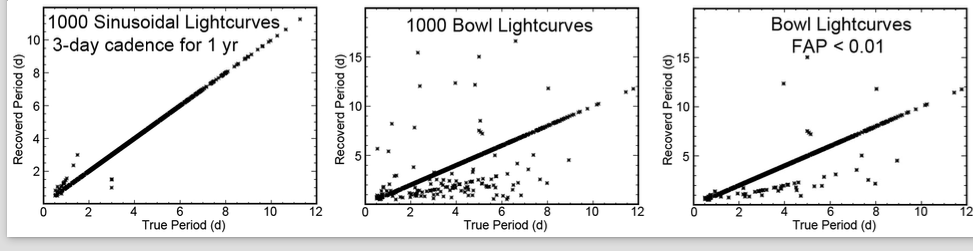
\includegraphics[width=5.32in]{figs/starFormation/tts1.pdf}
 \caption{Recovered period vs. true period for a sample of sinusoidal (left),
bowl-shaped (middle) and bowl-shaped with False Alarm Probability $<$ 0.01 (right),
assuming a 3-day cadence and one year of observing. What appears as a solid line are the
individual points with periods that are recovered correctly. The bowl-shaped curves are
more difficult to recover than the sinusoids, but the method is highly successful in both cases.}
   \label{tts1}
\end{center}
\end{figure}

\begin{figure}[b]
\vspace*{1.0 cm}
\begin{center}
 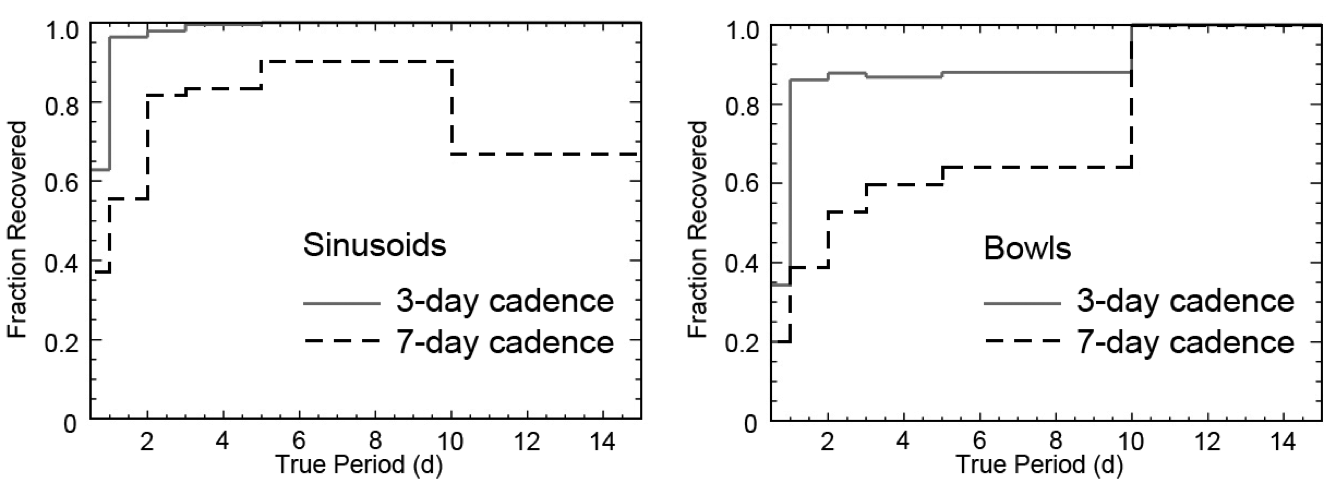
\includegraphics[width=5.32in]{figs/starFormation/tts2.pdf}
 \caption{ Fraction of periods recovered correctly for sinusoidal (left) and bowl light curves (right) for
3-day (solid line) and 7-day (dashed line) cadences over an observing period of one year.
A 3-day cadence is significantly better than a 7-day one. Over 98\%\ of sinusoidal, and 86\%\ of bowl
light curve periods are recovered successfully with the 3-day cadence. The percentages drop to about
82\%\ and 59\%\, respectively, for the 7-day cadence.
}
   \label{tts2}
\end{center}
\end{figure}

\begin{figure}[b]
\vspace*{1.0 cm}
\begin{center}
 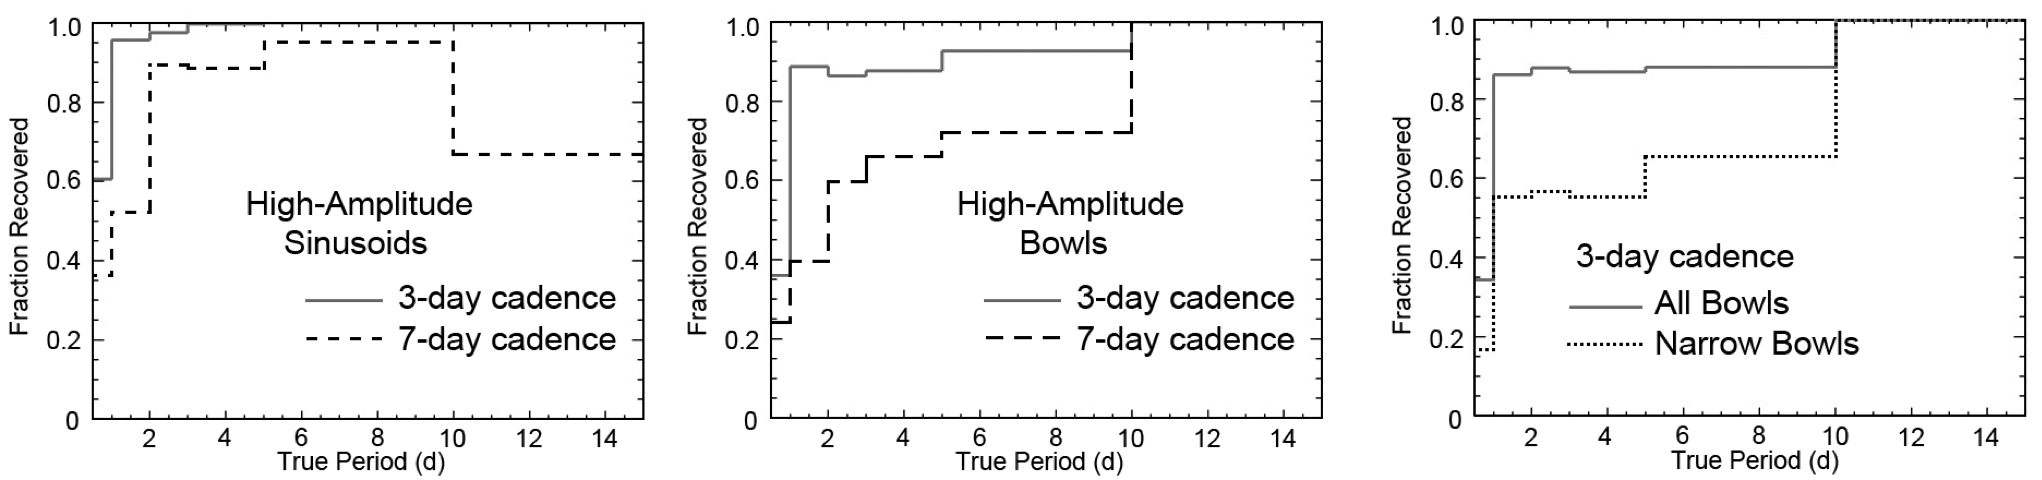
\includegraphics[width=5.32in]{figs/starFormation/tts3.pdf}
 \caption{Left and center: Same as Fig 2 but restricting the sample to amplitudes greater than 0.1 mag. The
method is only marginally more successful with the larger amplitude objects than it is with the entire sample.
Right: The narrowest 278 bowls have a significantly higher error rate than the entire sample does.
}
   \label{tts3}
\end{center}
\end{figure}

Overall, standard cadences of once every few days should suffice
to find most periodic T-Tauri stars that have periods $\gtrsim$ 3 days.
A dedicated campaign to observe star-forming regions
at time intervals of an hour or less is required to capture the shorter-period systems.
The r-filter should suffice for most objects, though some benefit will be had
by going to z to allow the more heavily-extincted sources to be observed.

{\bf C. Period Recovery for cTTs}

Complex irregular variations in cTTs lightcurves make it much more difficult,
and in many cases impossible to
recover periods in these systems. While sparse coverage of one observation every
few days is adequate for identifying sudden changes from accretion events, these
events to a large degree overwhelm low-amplitude periodic signatures. Even when
period searches yield a low false-alarm probability, the results are not necessarily
reliable. Results from Palomar Transient Factory surveys in the North American
Nebula \citep{Findeisen2013} and with Spitzer
\citep{Cody2014}
reveal several types of both short- and long-term variations including both bursting and
fading.  These observations emphasize how important it will be to have some
dense phase coverage as a reality check to ensure the reliability of
any periods recovered from sparse data in these objects, as well as to
follow the short-term variations that characterize accreting systems.

{\bf D. Discovery, Accretion and Extinction Events}

As we indicated above, any
cadence will uncover FU Ori and EX Ori events in all filters.
Periodic extinction events follow the same restrictions and
have the same requirements as rotational periods described in subsection B.

In order to assess the ability of LSST to identify and classify
eruptive variables (FUor/EXor), we construct
\autoref{table:pseudoForExor}, which shows a possible Figure of Merit for the
recovery by LSST of the distribution of EXor high-state duration in
outburst.

\begin{table}
\small
\begin{tabular}{c p{12cm}}
& {\it Figure of Merit for recovery of EXor high--state duration distribution}\\
\hline
1.  & Produce ASCII lightcurve for eruptive outburst \\
2.  & Initialise large array to store the maps of fraction detected as a function of duration and amplitude. \\
2.  & for {\it duration T} in range \{min, max\}:  \\
3.  & ~~~~ for {\it amplitude A} in range \{min, max\}: \\
4.  & ~~~~~~~~~~ run {\tt mafContrib/transientAsciiMetric} \\
5.  & ~~~~~~~~~~ store the spatial map of the fraction detected for this (A, T) pair \\
6.  & Initialise master arrays to hold the run of duration distribution measurements.\\
7. & Produce distribution of high--state durations and amplitudes from which the simulations will be drawn. \\
8.  & for {\it iDraw} in range \{1, nDraws\}:\\
9.  & ~~~~ construct model population with input duration distribution \\
10.  & ~~~~ Apply the stored metrics from 2-5 to measure fraction recovered \\
11.  & ~~~~ Characterize the duration distribution for this draw \\
12. & ~~~~ Fill the {\it iDraw}'th entry in the master arrays. \\
13. & {\bf FoM 1:} Compute the median and variance of the upper/lower quintiles. \\
14. & {\bf FoM 2:} Evaluate the bias between recovered and input high-state duration. \\
\hline
\end{tabular}
\caption{Steps for Figure of Merit recovering the distribution
  for the duration of EXor high states.}
\label{table:pseudoForExor}
\end{table}

% --------------------------------------------------------------------

\subsection{Summary and Recommendations}
\label{sec:\secname:discussion}

{\bf Performance for Nominal Cadences}

Nominal cadences that return to a star-forming region every 3-4 days
will suffice to determine rotation periods for $\sim$ 90\%\ of the
young stars within the magnitude limits of LSST.
These cadences are also adequate to detect major episodic
accretion events like FU Ori's and EX Ori's. However, a more focused
annual campaign of about a week duration is necessary to optimize
period recovery and angular momentum studies of young stars.

{\bf The Need for Annual Dense Coverage of a Few Selected Regions}

Occasional dense coverage of targeted regions is the only way to
get quantitative information on short-term accretion and flare
activity.  Dense coverage also removes degeneracies
for periodic variables that have periods less than a day, and is
the only way to provide a sanity check on any periods recovered for
cTTs, which have complex irregular light variations.
Comparing longevities of starspots across the mass ranges of young
stars requires two well-sampled lightcurves separated by large
time intervals.  The embedded and Classical T Tauri stars also undergo
significant and rapid color changes due to both accretion processes
and extinction variations, so it is important
to include multiple filters in any dense coverage campaign.

These goals can be accomplished by having a week every year where
one or more selected fields are observed once every 30 minutes in u, r and z.
A young star with a 2-day period sampled every 30 minutes provides a
data point every 0.01 in phase. For the best-case scenario, observing for 7 nights
and 10 hours per night would yield 140 photometric points in each filter.
Depending on the period aliasing, this coverage should populate the
phases well enough to identify most of the large starspots on the stellar photospheres.

At the beginning of LSST operations we argue that a targeted test field
be observed in this manner to illustrate what can be done with LSST in this mode.
Combining a densely-packed short-interval
dataset with a sparse but long baseline study maxmizes the scientific return
for both methods, and allows LSST to address all of the accretion and
rotational variability associated with young stars.

\subsection{Conclusions}
\begin{description}
\item[Q1:] {\it Does the science case place any constraints on the
tradeoff between the sky coverage and coadded depth? For example, should
the sky coverage be maximized (to $\sim$30,000 deg$^2$, as e.g., in
Pan-STARRS) or the number of detected galaxies (the current baseline 
of 18,000 deg$^2$)?}
%
\item[A1:] 
Most young stars congregate into clusters in specific regions, though there is an older
population that is more distributed. The vast majority are within $\sim$ 25 degrees of the
galactic plane. As long as that swath of sky is covered to the degree possible from Chile,
the survey will provide the young star community with the monitoring capability needed to
identify transient outbursts and to study periodic and aperiodic phenomena in young stars.
While it may be useful to have deep coadded images of some regions, for example, to identify
optical counterparts to X-ray point sources, dust extinction typically limits such efforts
in the optical towards most regions of interest.  Hence, deep coadded frames are a secondary
priority.

\item[Q2:] {\it Does the science case place any constraints on the
tradeoff between uniformity of sampling and frequency of  sampling? For
example, a rolling cadence can provide enhanced sample rates over a part
of the survey or the entire survey for a designated time at the cost of
reduced sample rate the rest of the time (while maintaining the nominal
total visit counts).}

\item[A2:] 
We discussed cadences in some detail above. To obtain the best constraints on periods, a time-intensive
($\sim$ one week/year) campaign on a few selected regions is warranted. Nominal coverage over the
galactic plane will suffice to identify eruptive variables.

\item[Q3:] {\it Does the science case place any constraints on the
tradeoff between the single-visit depth and the number of visits
(especially in the $u$-band where longer exposures would minimize the
impact of the readout noise)?}

\item[A3:] 
This item is discussed in section A above. In young stars, the u-band is particularly useful
as a measure of accretion. At the same time, for period determinations, denser cadences produce
fewer problems with aliasing for the typical young star variable with a rotation period between
a day and two weeks.

\item[Q4:] {\it Does the science case place any constraints on the
Galactic plane coverage (spatial coverage, temporal sampling, visits per
band)?}

\item[A4:] 
A nominal sampling of once every few days will suffice to identify interesting
eruptive variables as long as the galactic plane coverage is good (item A1).
However, a sparse temporal sampling such as this will make it difficult to interpret
the lightcurves of the tens of thousands of T Tauri stars observed by LSST. A single
week's campaign of dense sampling, e.g., 2-3 times per night, of targeted regions
will greatly improve our ability to separate periodic variables from aperiodic ones. 
Knowing the rotation periods of thousands of young stars within a given star forming
region will be a major contribution that LSST makes to this field of research. Such data
will allow us to learn how angular momentum is distributed among newborn
stars, whether it changes with mass and location in the cloud, 
and how it varies as the stars age. 

\item[Q5:] {\it Does the science case place any constraints on the
fraction of observing time allocated to each band?}

\item[A5:] 
In the case we made above for dense sampling, we argued for z, r, and u. The
u-band allows us to follow mass accretion variability, while r and z (for most
objects) will be dominated by photospheric flux. The r-z color is an important
constraint for models of star spots. More colors are always useful, but having
a photospheric color index plus one accretion measure are the science drivers 
for filter choices. Once u, r, and z are observed, having higher cadences
is preferable to having more bands.
The exposure times and magnitudes for typical objects are described in section A
above.

\item[Q6:] {\it Does the science case place any constraints on the
cadence for deep drilling fields?}

\item[A6:] 
Absolutely. We argue in the `Summary and Recommendations' section above
for the advantages of a single week of denser monitoring for specific
regions, with the goal of having several observations per night, separated
in time by at least an hour from one another. The goal here is to provide
some basis in reality for interpreting the irregular lightcurves of young
stars, which also typically have a periodic component. Depending on the longevity of
the star spots, a period might be obvious in high-cadence data taken over
a week, but disappear over a year if some spots vanish and others form. 

\item[Q7:] {\it Assuming two visits per night, would the science case
benefit if they are obtained in the same band or not?}

\item[A7:] 
If the data are taken in the same band
it means better sampling for periods. With different bands it means a lightcurve in two bands,
which is also useful. It's probably a wash, and we can follow whatever the drivers are for the
other science cases of LSST.

\item[Q8:] {\it Will the case science benefit from a special cadence
prescription during commissioning or early in the survey, such as:
acquiring a full 10-year count of visits for a small area (either in all
the bands or in a  selected set); a greatly enhanced cadence for a small
area?}

\item[A8:] 
Yes, definitely. We ought to see what we can get out of a dedicated week-long
LSST cadence on specific regions. If the results are impressive we follow up 
on different regions every year (or even return to the same regions).

\item[Q9:] {\it Does the science case place any constraints on the
sampling of observing conditions (e.g., seeing, dark sky, airmass),
possibly as a function of band, etc.?}

\item[A9:] 

Better seeing helps with unresolved binaries and for regions where contamination comes
into play, for example, in the plane but away from dark clouds. Some of the fainter objects
will be affected if the Moon is very bright and close. However generally these constraints
are probably in a 'typical' category and will not affect the design of the survey.

\item[Q10:] {\it Does the case have science drivers that would require
real-time exposure time optimization to obtain nearly constant
single-visit limiting depth?}

\item[A10:] 
No.

\end{description}

% ====================================================================

% bibtems need pushing into the relevant file!

%Hartmann \& Kenyon 1996, ARA\&A, 34, 207 \\
%Herbig et al. 2001, PASP, 113, 1547 \\
%Herbig 1977, ApJ, 217, 693 \\
%Aspin et al. 2009, ApJ, 692L, 67 \\
%Hodapp et al. 1996, ApJ, 468, 861 \\
%McGehee et al. 2004, ApJ, 616, 1058 \\

%\bibitem[Affer et al. (2013)]{Affer13}
%{Affer, L., Micela, G., Favata, F., Flaccomio, E., \& Bouvier, J.} 2013
%\textit{MNRAS}, 430, 1433

%\bibitem[Alencar al. (2010)]{CoRoT}
%{Alencar, S. H. P. et al.} 2010,
%\textit{A\&A}, 519, A88

%\bibitem[Cody al. (2014)]{cody14}
%Cody, A., et al.
%{Cody, A. et al.} 2014,
%\textit{AJ}, 147, 82

%\bibitem[Grankin al. (2008)]{ROTOR}
%\bibitem[Findeisen al. (2013)]{findeisen13}
%Findeisen, K., Hillenbrand, L., Ofek, E., Levitan, D., Sesar, B., Laher, R., \& Surace, J.
%{Findeisen, K. et al.} 2013,
%\textit{ApJ}, 768, 93

%\bibitem[Grankin al. (2008)]{ROTOR}
%{Grankin, K. N., Bouvier, J., Herbst, W., \& Melnikov, S. Yu.} 2008,
%\textit{A\&A}, 479, 827

%\bibitem[Horne \& Baliunas (1986)]{Scargle}
%{Horne, J. H. \& Baliunas, S.} 1986, \textit{ApJ}, 302, 757

\navigationbar


% --------------------------------------------------------------------

\input{Variables/future.tex}

% --------------------------------------------------------------------
